\documentclass[12pt, a4paper]{article}
\usepackage{caption}
\usepackage{graphicx}
\usepackage{hyperref}
\hypersetup{
    colorlinks,
    citecolor=black,
    filecolor=black,
    linkcolor=black,
    urlcolor=black
}
\usepackage{tikz-network}
\usepackage{amsmath, amsfonts, amssymb, amsthm}
\usepackage{algpseudocode}
\usepackage{algorithm}
\title{Linear algebra}
\date{2022}
\author{Kristoffer Klokker}

\usepackage{xcolor,listings}
\usepackage{textcomp}
\usepackage{color}
\usepackage{listings}
\definecolor{codegreen}{rgb}{0,0.6,0}
\definecolor{codegray}{rgb}{0.5,0.5,0.5}
\definecolor{codepurple}{HTML}{C42043}
\definecolor{backcolour}{HTML}{F2F2F2}
\definecolor{bookColor}{cmyk}{0,0,0,0.90}  
\color{bookColor}

\lstset{upquote=true}

\lstdefinestyle{mystyle}{
    backgroundcolor=\color{backcolour},   
    commentstyle=\color{codegreen},
    keywordstyle=\color{codepurple},
    numberstyle=\numberstyle,
    stringstyle=\color{codepurple},
    basicstyle=\footnotesize\ttfamily,
    breakatwhitespace=false,
    breaklines=true,
    captionpos=b,
    keepspaces=true,
    numbers=left,
    numbersep=10pt,
    showspaces=false,
    showstringspaces=false,
    showtabs=false,
    tabsize=3,
}
\lstset{style=mystyle}
\usepackage{zref-base}

\makeatletter
\newcounter{mylstlisting}
\newcounter{mylstlines}
\lst@AddToHook{PreSet}{%
  \stepcounter{mylstlisting}%
  \ifnum\mylstlines=1\relax
    \lstset{numbers=none}
  \else
    \lstset{numbers=left}
  \fi
  \setcounter{mylstlines}{0}%
}
\lst@AddToHook{EveryPar}{%
  \stepcounter{mylstlines}%
}
\lst@AddToHook{ExitVars}{%
  \begingroup
    \zref@wrapper@immediate{%
      \zref@setcurrent{default}{\the\value{mylstlines}}%
      \zref@labelbyprops{mylstlines\the\value{mylstlisting}}{default}%
    }%
  \endgroup
}

% \mylstlines print number of lines inside listing caption
\newcommand*{\mylstlines}{%
  \zref@extractdefault{mylstlines\the\value{mylstlisting}}{default}{0}%
}
\makeatother


\newcommand\numberstyle[1]{%
    \footnotesize
    \color{codegray}%
    \ttfamily
    \ifnum#1<10 0\fi#1 |%
}


\begin{document}
	\maketitle
	\clearpage
	\tableofcontents
	\clearpage
	\section{Systems of linear Systems of Linear Equations}
		A system of linear equations are multiple equations containing unknows which are shared. Ex.
		\begin{alignat*}{4}
		   2x & {}+{} &  y & {}+{} & 3z & {}={} & 10 \\
		    x & {}+{} &  y & {}+{} &  z & {}={} &  6 \\
		    x & {}+{} & 3y & {}+{} & 2z & {}={} & 13
		\end{alignat*}
		The same system may be wirtten in form of a matrix\\
		$$\begin{bmatrix}
			2 & 1 & 3 & 10\\
			1 & 1 & 1 & 6\\
			1 & 3 & 2 & 13
		\end{bmatrix}$$
		When solving a system their may be
		\begin{itemize}
			\item No solutions - No possible value can be assigned to the variable such all equation are true (inconsistent)
			\item One solution - A combination of values can be assigned to make every equation true (consistent)
			\item Infinite solutions - One or more unknows may have an infinite amount of possible assignable values (consistent)
		\end{itemize}
		By transforming a system of equations to a matrice, the following row operations can be performed:
		\begin{itemize}
			\item Multiply a row through by a nonzero constant.
			\item Interchange two rows.
			\item Add a constant times one row to another.
		\end{itemize}
		\subsection{Gauss-Jordan Elimination}
			Solving a system of equation in a matrice, can be done such the matrice has the following requirements
			\begin{itemize}
				\item If the row contain nothing but zeroes the first number should be a 1, called the leading 1.
				\item If a row is made of nothing but zeroes it should be grouped at the bottom
				\item In two rows the top row should contain a leading 1 further to the left than the bottom
				\item Each column which contains a leading 1, every number in the same column below should be 0
			\end{itemize}
			This form is called row echelon form.\\
			The solution may also be written as:
			$$\{(x_1=4,x_2=6,x_3=t,x_4=v,x_5=1)|t\in \mathbb{R} \}$$
			Where variables means they can be any possible asignment or a function with given restrictions, called free variables.\\
			In case of the leading 1 column is zero both above and underneath the matrice is in reduced echlon form.\\[4mm]
			To make a matrice into echoleon form the following algorithm can be used:\\
			\begin{enumerate}
				\item Locate the leftmost column that does not consist entruely of zeros and exhange it to the top
				\item Multiply the top row by $\frac{1}{a}$ where $a$ is the leading number in the row
				\item subtract top row from every other below row, such the top row is the only non zero value in the column
				\item Repeat 2 and 3 but ignore the top row and let the second top row be the top
			\end{enumerate}
			To reduce the echloen form, from the bottom the bottom row is added to the above rows until the leading 1 is the only in the column. This is repeated until the top is reached.\\
			A homogeneous linear system are systems which all constant (right part of equal) are 0 and the trivial solution (all variables are assigned 0) are a possible solution.\\
			A free variable is the term for a variable which can be assigned multiple values. The number of free variables wil lbe equal to the number of variables minus zero rows.\\
			In a homogenous linear system if the number of unknows exceed the number of equation there will be an infinite amount of solutions.\\
			Back substitution is a method taking the echoloen form and starting from the bottom isolating the leading variable and substituting it upwards.\\
			A echoloen form is not unique to a system but a reduced echoloen form is unique and the number of zero rows will be unique.
		\subsection{Matrices and Matrix operations}
			A matrix is a rectangular array of numbers called entries.\\
			The size of a matrix is written as rows x columns\\
			A single row matrix is alled a row vector and single column is called column vector.\\
			Standard basis  is the set of column vectors in a identity matrix.\\
			Variables in matrices are called scalars and unless stated is in the realm of real numbers.\\
			When refering to a number in the matrix A it will be $a_{row\;column}$ and the value can be found by $(A)_{row\;column}$\\
			A matrix scalar matrix can be written as $A=[a_{ij}]_{m\times n}$ the $m\times n$ is optional if the size matters.\\
			\subsubsection{Matrix operations}
				Addition/subtraction - every number in corresponding entries are added/subtracted.\\
				Addtion and subtraction can not be done on two different sized matrices.\\[4mm]
				Multiplying a matrix with a scalar, is done by multiplying the scalar on every entry.\\
				For multiplying two matrices an entry is found by $a_{ij}=\sum\limits_{t=0}^n b_{i(j+t)}\cdot c_{(i+t)j}$ where $n$ is the size of row size of matrix $b$ and column size of matrix $c$, if this value does not match the two matrices can not be multiplied.\\
				The reuslting product matrix of $a = b \times c$ will have the size rows = c columns and columns = b rows\\[4mm]
				Partioning a matrix is the act of splitting it into a smaller valid matrices. This can be used if only certain entries are wanted for a matrix multiplication\\
				Linear combinations are an array of matrices (length $n$) of the same size matrix $A$ and an array of scalars (length $n$) $c$ computed as $\sum\limits_{i=o}^n A_i\cdot c_i$\\
				Multiplying a vector row and a matrix (with approprate lengths) can therefore be expressed as an linear combination.\\
				Column row expansion is the act of splitting two matrices being multiplied into rows and columns, and then taking the sum of each product of row and column, and thus getting the muiltiplied matrix.\\[4mm]
				Matrix form of linear system is the act of expressing a linear system in the form of matrix $A$ containing all coefficients, matrix $X$ containing a column vector of all unknown variables, and matrix $B$ which is a column vector of all results of the linear system. in this way the linear system can be expressed as $AX=B$\\
				Tranposing a matrix is flipping column and rows such in matrix $A$ the entry $a_{ij}$ is now entry $a_{ji}$ in the matrix $A^T$.\\
				A trace operation of matrix $A$ is taking the addition of the diagonal line called $tr(A)$, can only be performed on square matrices.\\
				The trace of a square matrix is defined as $tr(A)=a_{11}+a_{22}+...+a_{nn}$ or $tr(A)=\sum\limits_{i=0}^n a_{ii}$\\
				For the trace the following is true
				\begin{itemize}
					\item $tr(A^T)=tr(A)$
					\item $tr(A\pm B)=tr(A)\pm tr(B)$
					\item $tr(cA)=c\cdot tr(A)$
					\item $tr(AB)=tr(BA)$
				\end{itemize}
				The matrix polynomials are a way of describing multiple equations in matrix form by\\
				If $A$ contains all the coefficients, $X$ contains all variables in a column vector, and $B$ contains all constant the equations are equal to in a column vector.\\
				Then the equations can be described as  $A\cdot X=B$
		\subsection{Inverses}
			For matrix operations are the following true, if the size allows for it
			\begin{itemize}
				\item Commutative law for matrix addition - $A + B = B + A$
				\item Associative law for matrix addition - $A + ( B + C) = (A+B)+C$
				\item Associative law for matrix multiplication - $A(BC)=(AB)C$\\
				\item Left and Right distributive law - $A(B+C)=AB+AC$
			\end{itemize}
			Zero matrices are matrices consisting of only zeros and are denoted by $0_{m\times n}$\\
			Identity matrix $I$ is the matrix containing 1's on the diagonal, and has the proberty that if multiplies by $A$ the product is $A$.\\
			The inverse matrix $A^{-1}$ is the matrix $B$ to the square $A$ if $AB=I$, and $A$ is said to be invertible. If $B$ does not exist $A$ is singular\\
			Only one inverse exist to a matrix.\\
			For two inverse matrices is the following true $B^{-1}A^{-1}=(AB)^{-1}$.\\
			Powers if a matrix is defined as expected, and for $A^0=I$ and if $A$ is invertible then $A^{-n}=(A^{-1})^n$\\
			$A^n$ is invertible and $(A^n)^{-1}=A^{-n}=(A^{-1})^n$\\
			Matrix pylonomials are inserting a matrix into a polynomial function.\\
			Transpose if the interchangning of rows in a matrix, and are expressed as $(A^T)^{-1}=(A^{-1})^T$.\\
			The transposed matrix has the follwoing properties:
			\begin{itemize}
				\item $(A^T)^T=A$
				\item $(A\pm B)^T=A^T\pm B^T$ 
				\item $(cA)^T=cA^T$
				\item $(AB)^T=B^TA^T$
			\end{itemize}
		\subsection{Determinants by cofactor expansion}
			Minor of entry $a_{ij}$ is denoted $M_{ij}$ and is defined as the determinant of the submatrix that remains when i row and j column is deleted.\\
			The cofactor $C_{ij}$ of $M_{ij}$ is defined as, if $i+j$ is even then $1^{i+j}M_{ij}$ and $(-1)^{i+j}M_{ij}$ if odd\\
			The determinant of an $n\times n$ matrix can be found either by a row or column in the following way:
			$$det(A)=a_{1j}C_{1j}+a_{2j}C_{2j}+...+a_{nj}C_{nj}$$
			This is via the column and by switching $i$ and $j$ it is by the row.\\
			Therefore making the definition recursive.\\
			If we make the function $f(i,j)=1 - ((i+j) \% 2 ) \cdot 2$ such it will be $-1$ when the sum of $i$ and $j$ is odd and $1$ when the sum is even.
			$$det(A)=a_{1j}f(1,j)^{1+j}M_{1j}+a_{2j}f(2,j)^{2+j}M_{2j}+...+a_{nj}f(n,j)^{n+j}M_{nj}$$
			if we also denote the function $g(A,i,j)$ to be a function which removes row $i$ and $j$\\
			Then we can make a true recursive definition.\\
			$$det(A)=a_{1j}f(1,j)^{1+j}det(g(A,1,j)+a_{2j}f(2,j)^{2+j}det(g(A,2,j)+...+a_{nj}f(n,j)^{n+j}det(g(A,n,j)$$
			Where for the 1x1 matrix $det([a_{11}])=a_{11}$
			If $A$ is triangular then $det(A)$ is equal to the product of the main diagonal.\\[4mm]
			It can also be noted that determination of the zero matrix is zero\\
			And for the transpose $det(A)=det(A^T)$\\[4mm]
			To make life easier row operation can be done such less operations are needed to find the determinant.\\
			When performning row operation the following is the for the $A$ matrix with size $n\times n$
			\begin{itemize}
				\item If $B$ is the result of a row or column in $A$ being multipled by a constant $k$ then $det(B)=k\cdot det(A)$
				\item if $B$ is the result of two rows or two columns being interchanged then $det(B)=-det(A)$
				\item if $B$ is the result of one row being multiplied and added to another row then $det(B)=det(A)$
			\end{itemize}
			For the special case where $A=I_n$ and $E$ is the result of an row operation on $A$ the follwing applies
			\begin{itemize}
				\item If $E$ is the result of multiplying a row with the constant $k$ which is not 0 then $det(E)=k$
				\item If $E$ is the result of interchaning two rows then $det(E)=-1$
				\item If $E$ is the result of adding a constant to a row and adding to another then $det(E)=1$
			\end{itemize}
			If $A$ has a row/column which is proportional to another then $det(A)=0$\\
			Reducing a matrix the echeloen, in doing so instead of reducing the a row by 1/ the leading value, the leading value is taken to the side, then the product of every value taken to the side will be equal to the determinant.\\
		\subsection{Properties of determinants}
			If $A$ is a $n\times n$ matrix and $C_{ij}$ is the cofactor of $A_{ij}$, then the matrix is called matrix of cofactors from $A$\\
			The transpose of the matrix of cofactors from $A$ is called adjoint of $A$
			\begin{itemize}
				\item $det(kA)=k^ndet(A)$
				\item $det(C)=det(A)+det(B)$  If A and B only differ in one row/column and C is equal to A and the the differ row/column sum
				\item $det(AB)=det(A)det(B)$ if both $A$ and $B$ are $n\times n$ matrices
				\item $A$ is only invertible if $det(A)\neq 0$
				\item If $A$ is invertible then $det(A^{-1})=\frac{1}{det(A)}$
				\item If $A$ is invertible then $A^{-1}=\frac{1}{det(A)}adj(A)$
			\end{itemize}
			In the system of linear equation $Ax=b$ then the solutions can be found by
			$$x_n=\frac{det(A_n)}{det(A)}$$
		\subsection{Matrix transformation}
			The matrix transformation is function $T_A(x)=A\cdot x$, which transforms the axis linearly, such origo stays in the same place.\\
			The function then takes a vector of length $n$ and multiply it / transforms it with a matrix of size $n\times n$\\
			The transformation which has the follwing proberties:
			\begin{itemize}
				\item $T_A(0)=0$ Origin stays in place
				\item $T_A(k\cdot x) = k\cdot T_A(x)$ 
				\item $T_A(x+y)=T_A(x)+T_A(y)$
				\item $T_A(x-y)=T_A(x)-T_A(y)$
			\end{itemize}
			To think of the matrix $A$ which the transformation use, it can be though of in the coordination system x,y,z $A$ would then be a 3x3 matrix.\\
			Each column then represent the standard basis for the axis. \\
			Such for the Cartesian (standard) coordination system, the matrix would be a 3x3 identity matrix.\\
			Generally speaking the identity matrix is also called to standard matrix\\[4mm]
			The transformation may also be composited together like $(T_B\cdot T_A)(x)=T_B(T_A(X))$\\
			Likewise multiplication the transformation is not commutative $T_A\cdot T_B\neq T_B \cdot T_A$\\
			The exception to this is rotation and reflection transformations.\\
			If $A$ is invertible then $T_A:R^n\rightarrow R^n$ $R^n$ is also invertible.\\
			This is written as $T_A^{-1}=T_{A^{-1}}$\\
			A linear transformation is when $T:\mathbb{R}^N\rightarrow\mathbb{R}^M$ statisfies the follwing linear conditions
			\begin{itemize}
				\item $T(k\cdot x) = k\cdot T(x)$
				\item $T(x+y)=T(x)+T(y)$
			\end{itemize}
		\subsection{Projections}
			A projection is a transformation to a lower dimension system.\\
			An orthogonal projections is a projection on a line, plane or the appropriate amount of dimensions.\\
	\section{Vector spaces}
		If $V$ defines all objects which are non empty then
		\begin{itemize}
			\item $u,v\in V\rightarrow v+u\in V$
			\item $u+v=v+u$
			\item $u+(v+w)=(u+v)+w$
			\item The zero vector exist called $0$ with the property $v+0=v$
			\item For each $u$ in $V$ exists a $-u$ such $u+(-u)=0$
			\item If $k$ is a scalar and $u$ is in $V$ then $uk$ is in $V$
			\item  $k(u+v)=ku+kv$
			\item $k(mu)=(km)u$
			\item $1u=u$
		\end{itemize}
		If an object satisfies all these axioms then we can classify a set of objects as being in the  vector space.\\
		Therefore $\mathbb{R}$ is in the vector space, $\mathbb{R}^n$ being the vector of real number length $n$ is in the vector space.\\
		Likewise $\mathbb{R}^{n\cdot m}$ matrix is in the vector space and even functions like the polynomial functions are in the vector space.\\
		\subsection{Subspaces}
			A subspace $W$ of $V$ is a subspace if $u$ and $v$ are in $W$ and $u+v$ is in $W$.\\
			And if $k$ is a scalar and $u$ is in $W$ then $ku$ is in $W$\\ 
		\subsection{Spanning sets}
			$w$ is said to be a linear combination if 
			$$w=k_1v_1+k_2v_2+...+k_rv_r$$
			Where $k$ is coefficients and $v$ is vectors in the vector space $V$.\\
			To say that the linear combination is spanning means by the given vectors a linear combination can be made such every vector is made in the space.\\
			So if $V$ is the vector space and $W\leq V$ a subspace such that $W=span\{w_1,...,w_n\}$ then the set is the spanning set of $W$\\
			To find if a vector can be expressed as a combination of two vectors, the two vectors is added with an unknown scalar at each vector in the addition.\\
			The expression can then be split up such for the vector of size $n$ there will be $n$ equation with $q$ unknowns equal to the amount of addition.\\
			\begin{align*}
				(9,2,7)&=k_1(1,2,-1)+k_2(6,4,2)\\
				&=(k_1+6k_2,2k_1+4k_2,-k_1+2k_2)\\[3mm]
				9&=k_1+6k_2\\
				2&=2k_1+4k_2\\
				77&=-k_1+2k_2\\[3mm]
				k_1&=-3\\
				k_2&=2
			\end{align*}\\
			This method can be more generalised by setting it up in a matrix form and instead of finding a single vector it can just be a general vector of variables, from which Gauss-Jordan elimination can be used to find if the solution is consistent.
			To test if a set of vectors span an entire space, they can be setup as a matrix and if the determinant is non zero then it spans the entire space.
		\subsection{Linearly independent}
			A set of vectors is set to be linearly idependent set if no vector in the set can be expressed as linear combination of other vectors in the set.\\
			A set is linearly independent if the only solution is $k_1=0,k_2=0,..k_r=0$
			$$k_1v_1+k_2v_2+...k_r+v_r=0$$
			Where $v$ is the vectors in the vector set.\\
			This is again tested in a matrix form using elimination.\\
			A set if non inifinite vectors that contains 0 is linearly dependent. - This can be seen by the zero coefficient test will result in 0 using any coefficient.\\
			A set with exactly two vectors which is not a scalar multiple of each other are linearly independent.\\
			If a set contains more vectors than the size of the vectors then the set is linearly dependent.\\[4mm]
			To test if a set of functions $f_1,f_2,...f_n$ are linearly dependent they must be continuous derivable to $n-1$.\\
			They can then be setup in a matrix of size $n\times n$ where the first row is the functions, the next is the function derived once, this continuous til $n-1$.\\
			If the determinant is not 0 on $(-\infty,\infty)$ then the fuctions form a linearly independent set of vectors.
		\subsection{Coordinates and basis}
			Coordinate system are defiend by the basic vectors, in a rectungular 2D system they are (0,1) and (1,0).\\
			They both describe the positive direction and the unit spacing between integers.\\
			A vector space $V$ is set to be finite-dimensional if there exist a finite set of vectors in $V$ which spans $V$.\\
			An infinite-demensional set has no such set which spans $V$.\\
			If $S$ is a set of vectors in a finite-dimensional vector space $V$ then $S$ is a basis for $V$ if:
			\begin{itemize}
				\item $S$ spans $V$
				\item $S$ is linearly independent
			\end{itemize}
			The basis for a vector space $V$ there will be a unique combination for every vector in $V$.\\
			In the ordered basis $S$ the coefficients in the linear combination is called the coordinates of $v$ relative to the basis $S$\\
			The vector made from the combination is called the coordinate vector of $v$ relative to $S$ and is denoted by $(v)_S=(c_1,c_2,...,c_n)$ called comma-delimted form and may be expressed in a column matrix called matrix form\\
		\subsection{Dimensions}
			For the vector space with $n$ dimensions:\\
			If a set in $V$ has fewer than $n$ vector then it does nat span $V$ - due to some dimension not being represented\\
			If a set in $V$ has more then $n$ vectors then it not linearly dependent \\
			$dim(V)$ is a function which gives the number of dimensions of $V$.\\
		\subsection{Change of basis}
			When changing coordinate system a vector $V$ will be changed in to $(v)_s$ is then is displayed in matrix form.\\
			Therefore the before coordinate is changed in the coefficients used to create the vector.\\
			Changing the basis can be described as a transformation matrix, which transform the old basis vectors into the new basis vectors.\\
			It is denoted by $P_{B\rightarrow B'}=[[u_1']_B|[u_2']_B|...|[u_n']_B]$ where $B$ is the old basis and $B'$ is the new basis\\
			It can here be observed that $P_{B\rightarrow B'}\cdot P_{B'\rightarrow B}=I$\\
			To find the transition matrix, a matrix can be made of [new basis|old basis] where the basis's are column vectors of the basis vectors.\\
			Then the matrix is reduced to echeloen form which results in [I|transistion matrix from old to new]
	\section{General Linear Transformation}
		If $T:V\rightarrow W$ is a mapping between vector spaces then T is a linear transformation if the two proberties hold
		\begin{itemize}
			\item $T(ku)=kT(u)$
			\item $T(u+v)=T(u)+T(v)$
		\end{itemize}
		It can here be observed that the following is true
		\begin{itemize}
			\item $T(0)=0$
			\item $T(u-v)=T(u)-T(v)$
			\item $T(-v)=-T(v)$
		\end{itemize}
		The mapping $I:v\rightarrow$ defined by $I(v)=v$ is the identity operator.\\
		Let $T:V\rightarrow W$ a linear transformation. If $S=\{v_1,v_2,...,v_n\}$ is the basis for $V$ then any vector in $V$ can be described as
		$$T(V)=c_1T(v_1)+c_2T(v_2)+...+c_nT(v_n)$$
		Where $c_1,c_2,...c_n$ are the coefficients required to express v as a linear combination of vector basis in $S$\\
		For the transformation $T:V\rightarrow W$ then the kernel denoted by $ker(T)$ is all vectors in $V$ which maps into $0$\\
		Given a set of vectors the range denoted $R(T)$ is the possible outcome given the set of vector inputs.\\
		The rank of a transformation is denoted by $rank(T)$ and is equal to the number of dimension in the transformation\\
		The Nullity of the transformation is denoted by $nullity(T)$ and is equal to the number of dimensions which is in the kernal.\\
		It can here be seen in the transformation $T:V\rightarrow W$ that $rank(T)+nullity(T)=dim(V)$\\
		A transformation is set to be one-to-one if it maps every distinct vector to a new distinct vector. - $ker(T)=\{0\}$\\
		A transformation $T: V\rightarrow W$ is set to be onto $W$ if every vector in $W$ can be obtained through a mapping of $V$\\
		$T_A$ is one-to-one only if the columns of $A$ are linearly independent- due to if not linearly independent the nullity would be more then 0\\[4mm]
		\begin{figure}
			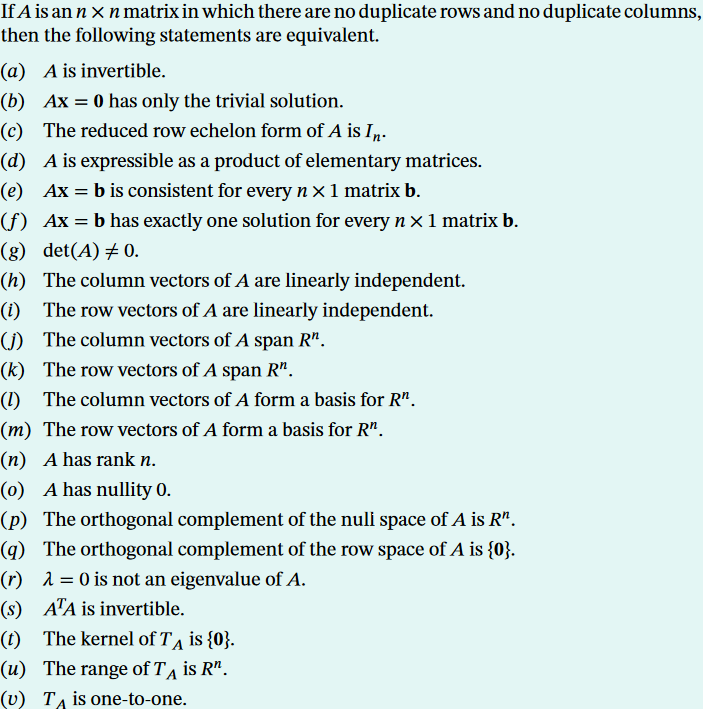
\includegraphics[width=300px]{assets/equivalentStatementsForInvertibleMatrix.png}
			\centering
			\caption{Equivalent statements for the invertible matrix}
		\end{figure}
		The inverse transformation is defined by if $T_A:V\rightarrow W$ then $T_{A^{-1}}=W\rightarrow V=T^{-1}$\\
		The row space is the space defiend by the rows. By reducing the transformation the number of none zero rows are the row space rank.\\
		The same goes for columns in the column space.\\
		It can here be observed that the row space and column space will ahve the same rank.
		\subsection{Matrices for general linear transformations}
			For the two vector spaces $V$ with basis $B$ and $W$ with basis $B'$. Here vector space $V$ is $n$ dimensions and $W$ is $m$ dimensions.\\ 
			Our goal is to find a matrix $A$ such a vector $x$ can be transformed from $V$ basis $B$ to $W$ basis $B'$ - $A[x]_B=[T(x)]_{B'}$\\
			If we have an $A\in\mathbb{M}_{m,n}(\mathbb{R})$ then $T(x)$ can be computed in the following steps
			\begin{enumerate}
				\item First compute $[x]_B\in \mathbb{R}^n$
				\item Then compute $A\cdot [x]_b\in \mathbb{R}^m$
				\item Reconstruct $T(X)$ from its $B'$ coordinates $[T(x)]_{B'}=A\cdot [x]_B$
			\end{enumerate}
			To find $A$ we can do the following
			\begin{enumerate}
				\item Write $B=\{u_1,...,u_n\}$ and $B'=\{v_1,...,v_m\}$
				\item Then $A=[[T(u_1)]_{B'}|...|[T(u_n)]_{B'}]\in\mathbb{M}_{m,n}(\mathbb{R})$
			\end{enumerate}
			The matrix $A$ is denoted $[T]_{B',B}$ and the order is choosen such $[T(x)]_{B'}=[T]_{B',B}\cdot [x]_B$\\
			This is caleld matrix of $T$ relatiove to $B$ and $B'$\\
			
		\subsection{Composition}
			The transformation of $T_1:U\rightarrow V$ and $T_2:V\rightarrow W$ can be combined to the linear transformation $(T_1\cdot T_2):U\rightarrow W$\\
			This is called the composition of the two transformations.\\
			This may again also be chained with other transformations.
			The composition will be linear and if both transformation is one-to-one then the composition is also one-to-one.\\
			If both transformations are isomorphisms then the composition and the inverse of the composition are isomorphisms\\
		\subsection{Isomorphism}
			A transformation $T:V\rightarrow W$ which is both one-to-one and onto is isomorphism, and $W$ is isomorphic to $V$ written as $W\simeq V$\\
			Therefore there will exist an inverse transformation such $T^{-1}\cdot T(v)=v$\\
			Two vector spaces are isomorphic iff they have the same dimension\\
		\subsection{Similarity}
			To find a transformation in bassis $B$ in another basis $B'$ then $[T]_{B'}=P^{-1}_{B'\rightarrow B}\cdot [T]_B\cdot P_{B'\rightarrow B}$
			It can then be said that $[T]_{B'}$ and $T_{B}$ is similar.
	\section{Eigenvalues and eigenvectors}
		An eigenvector is vector which only get scaled in a transformation, which is not a zero vector.\\
		This scaled value is the eigenvalue.\\
		$$Ax=\lambda x$$
		Where $x$ is the eigen vector, $A$ is a transformation and $\lambda$ is the eigenvalue.\\
		For the matrix $A$ it will be invertible only if $\lambda =0$ is not an eigenvalue of $A$.
		\subsection{Finding eigenvalues}
			To find an eigenvalue of a transformation, first it can be rewritten as
			$$Ax=\lambda\cdot I x$$
			Such it is matrix multiplcation on both sides and it can therefore be reduced
			$$(\lambda \cdot I-A)x=0$$
			Then an value for $\lambda$ can be found such the matrix in the parenthese will be linearly dependent.\\
			When the matrix is linear dependent, this makes it possible for there to exists an eigenvector of which the first equation holds true.\\
			When expanding $(\lambda\cdot I-A)$ it is known as the characteristic polynomial denoted $p(\lambda)$\\
			This polynomial is then solved to find the eigenvalues\\[4mm]
			An easy way to find eigenvalues for a 2x2 is by the formula
			$$\lambda=m\pm\sqrt{m^2-p}$$
			Where $m$ is the mean of the diagonal and $p$ is the determinant.\\[4mm]
			In case of an upper triangle or lower triangle the diagonal is the eigen values.\\
		\subsection{Finding eigenvectors}
			To find the eigenvector first the eigen values have to be known.\\
			Then the equation
			$$(\lambda\cdot I-A)\times x=0$$
			Where $x$ is the matrix of same size of $A$'s row and 0 is representing the zero vector.\\
			Then a system of equation can be made and solved for. \\
			The solutions can then be inserted in $x$ to find the eigenvector.
		\subsection{Diagonalization}
			Diagonalization describes the relation between eigenvalues, eigenvalues and the original vector
			$$A=XDX^{-1}$$
			Where $A$ is an matrix square with eigen values $\lambda_1,\lambda_2,...$\\
			$X$ is the matrix consisting of the eigenvectors $[x_1,x_2,...]$ which all are linear independent\\
			$D$ is the matrix consisting of 0's and the eigenvalues on the diagonal in the same order as the eigenvectors for $X$.\\[4mm]
			In general the diagonalization where $B=P^{-1}AP$ it is said that $B$ and $A$ are similar and will share many similarities and proberties.\\
			Diagnonalization is usefull since the eigenvalue to the power of the integer c is the eigenvalue to $A$ to the power of c\\
			So the transformation using $X$ can be used to to transform $D$ to the wanted power
	\section{Angles}
		To find angles for objects the formula
		$$\cos\theta = \frac{<u,v>}{||u||||v||}$$
		Where $<u,v>$ is the inner product, which is a extension of dot product. Found by taking $a_1b_1+a_2b_2+...a_nb_n$.\\
		$||u||$ is the length of $u$ found by taking $\sqrt{a_1^2+a_2^2+...+a_n^2}$.\\
		The innerproduct and length has to following proberties
		\begin{itemize}
			\item $<u,v>^2\leq <u,u><v,v>$
			\item $<u,v>^2\leq ||u||^2||v||^2$
			\item $||u+v||\leq ||u||+||v||$
			\item $d(u,v)\leq d(u,w)+d(w,v)$ where $d$ is the distance function
			\item $<u,v>=0$ the angle will be $90^\circ$ there the objects are orthogonal
			\item $||u+v||^2=||u||^2+||v||^2$
		\end{itemize}
		Orthogonal complements denoted $W^\perp$ are orthogonal objects for a subspace $W$ of $V$.\\
		Ex. in $R^3$ and the subspace describing a plane the orthogonal complement is vector of which the whole plane the orthogonal to.\\
		Therefore $W\cap W^\perp=\{0\}$ and $(W^\perp)^\perp=W$\\
		\subsection{Orthonormal basis}
			Orthonormal is the set of vectors in norm 1 which are orthogonal to an object.\\
			By norm 1, it means that every value in the vector is divided by the length of the vector.\\
			The orthonormal form can be seen to be linear independent and therefore a basis for $V$.\\
			To then find a vector $u$ in the basis, it can be found as
			$$u=\frac{<u,v_1>}{||v_1||^2}v_1+\frac{<u,v_2>}{||v_2||^2}v_2+...+\frac{<u,v_n>}{||v_n||^2}v_n$$
			Or just by 
			$$u=<u,v_1>v_1+<u,v_2>v_2+...+<u,v_n>v_n$$\\[4mm]
			If $W$ is a finite dimensional subspace of innter product space $V$, then every vector $u$ in $V$ can be descirbed by\\
			$$u=w_1+w^\perp$$
			Where $w_1$ is in $W$\\
			The projected vector $u$ is found by a linear combination of the basis vectors.
		\subsection{Gram-Schmidt process for finding orthonormal basis}
			The gram-schmidt process works by taking an orginal basis and turning it into orthogonal basis.\\
			For the basis $B=\{b_1,b_2,...,b_n\}$ to the orthogonal basis $U=\{u_1,u_2,...,u_n\}$ it can be done by
			$$u_k=b_k-\sum\limits_{i=i}^{k-1}\frac{<b_k,u_i}{|u_i|^2}u_i$$
			Therefore mkaing the first three terms
			\begin{align}
				u_1=b_1\\
				u_2=b_2-\frac{<b_2,u_1>}{|u_1|^2}u_1\\
				u_3=b_3-\frac{<b_3,u_1>}{|u_1|^2}u_1-\frac{<b_3,u_2>}{|u_2|^2}u_2
			\end{align}
		\subsection{Orthogonal matrices}
			A matrice which inverse is equal to the transpose is said to be orthogonal.\\
			$$AA^T=A^A=I$$
			$$A^{-1}=A^T$$
			It can be seen that if $A$ is orthogonal the row and column vectors of $A$ form an orthonormal set in $R^n$ with the euclidean inner product\\
			A product of orthogonal matrices is orthogonal.\\
			if $A$ is orthogonal then $det(A)=1 \lor det(A)=-1$\\
			$||Ax||=||x||$ for all $x$ in $R^n$ and $Ax\cdot Ay=x\cdot y$ for all $x$ and $y$ in $R^n$	
		\subsection{Orthogonal diagonalization}
			If $A$ and $B$ are square matrices, thenthey are  orthogonally similar matrices, if there exists an orthogonal matrix $P$ where $B=P^TAP$ and therefore $A=PBP^T$\\
			$P^TAP=D$ $P$ orthogonally diagonalizes and $A$ is orthogonally diagonalizable\\
			It can be seen that $A$ must be symmetric if it is orthogonally diagonalizable, and $A$ has an orthonormal set of $n$ eigenvectors.\\[4mm]
			To find the orthogonal diagonalization, first the each eigenspace is found and the gram schmidt process is applied to find basis for each eigenvector.\\
			Then a matrix $P$ is constructed from the eigenvectors in the columns. The diagonalization will then have the eigenvalues in the diagonal in the same order as the column vectors.\\[4mm]
			The spectral decomposition comes from $A=PDP^T$ which can be written as $A=\lambda_1u_1u_1^T+\lambda_2u_2u_2^T+\lambda_nu_nu_n^T$\\
			It can be seen that multiplying a vector $x$ to $A$, the result can be found by multiplying $x$ into each $\lambda uu^T$.\\
			There can for $D$ be found matrices in the form of an upper right triagnle denoted $S$ and in the form of upper right triangle plus an extra diagonal denoted $H$.\\
			These forms can help reduce the number of operations in algorithms.
			
			
		
				
\end{document}

